\section{Evaluation}
\label{sec:eval}

In this section, we use simulations to characterize the performance of each of our three recovery algorithms in terms of message and time overhead. 
Our goal is to illustrate the relative performance of our recovery algorithms over different topology types (e.g., \er graphs, Internet-like graphs) and
different network conditions (e.g., fixed link costs, changing link costs).
We evaluate recovery after a single compromised node has distributed false routing state.
%We count the number of messages required for nodes to find valid routing paths and count the number timesteps (epochs) for each algorithm to converge.

We build a custom simulator with a synchronous communication model: nodes send and receive messages at fixed epochs.  In each epoch, a node receives a
message from all its neighbors and performs its local computation.  In
the next epoch, the node sends a message (if needed).   All algorithms
are deterministic under this communication model.
The synchronous communication model, although simple, yields
interesting insights into the performance of each of the recovery
algorithms. Evaluation of our algorithms using a more general
asynchronous communication model is currently under
investigation. However, we believe an asynchronous implementation
will demonstrate similar trends.  

We simulate the following scenario:

\begin{enumerate}
	\item Before $t'$, $\forall v \in V$ \minvv and \dmatrixv are correctly computed.

	\item At time $t'$, \bad is compromised and advertises a \badvector (a vector with a cost of $1$ to \emph{every} node in the network) to its neighboring nodes.

	\item \badvector spreads for a specified number of hops (this varies by experiment).  Variable $k$ refers to the number of hops that \badvector has spread.

	\item At time $t$, some node $v \in V$ notifies all $v \in adj($\bads$)$ that \bad was compromised. 
	{\footnote { \small For \cpr this node also indicates the time, $t'$, \bad was compromised.}} 

\end{enumerate}
The message and time overhead are measured in step (4) above. The pre-computation common to all three recovery algorithms, described in Section \ref{subsec:preprocess},
is not counted towards message and time overhead.


\subsection{Fixed Link Weight Experiments}
\label{subsec:fixed}

In the next three experiments, we evaluate our recovery algorithms over different topology types in the case of fixed link costs.

\subsubsection{Experiment 1 - \er Graphs with Fixed Unit Link Weights}
\label{subsubsec:expt1}

We start with a simplified experiment setting to measure the 
 message and time overhead incurred by each of the recovery
 algorithms. In particular, we consider 
Erd\"{o}s-R\'enyi graphs with parameters $n$ and $p$. Further, the
link weight of each edge in the graph is set to 50.
$n$ is the number of graph nodes and $p$ is the probability that link $(i,j)$ exists where $i,j \in V$. We iterate over different values of $k$. For each $k$, we 
generate an Erd\"{o}s-R\'enyi graph, $G = (V,E)$, with parameters $n$ and $p$. Then we select a $v \in V$ uniformly at random and simulate the scenario described above, 
using $v$ as the compromised node. In total we sample $20$ unique nodes for each $G$.
We set $n=100$, $p=\{0.05,0.15,0.25, 0.25\}$, and let $k=\{1,2,
... 10\}$. Each data point is an average over $600$ runs ($20$ runs over 
$30$ topologies).  We then plot the $90 \%$ confidence interval.

For each of our recovery algorithms, Figure \ref{fig:msg} shows the
message overhead for different values of $k$. %The $90 \%$ confidence interval is shown.
We omit the $p=0.25$ figure because it shows the same trends as $p=0.15$ \cite{Tech}. 

\begin{figure*}[t]
\centering
\subfigure[{$p=0.05$, diameter=$6.14$}]{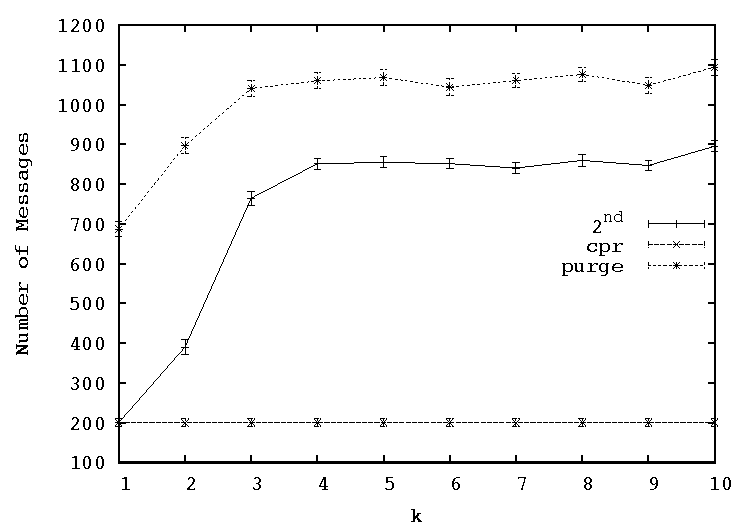
\includegraphics[width=0.32\textwidth]{figs/synch/msg5.pdf}}
\subfigure[{$p=0.15$, diameter=$3.01$}]{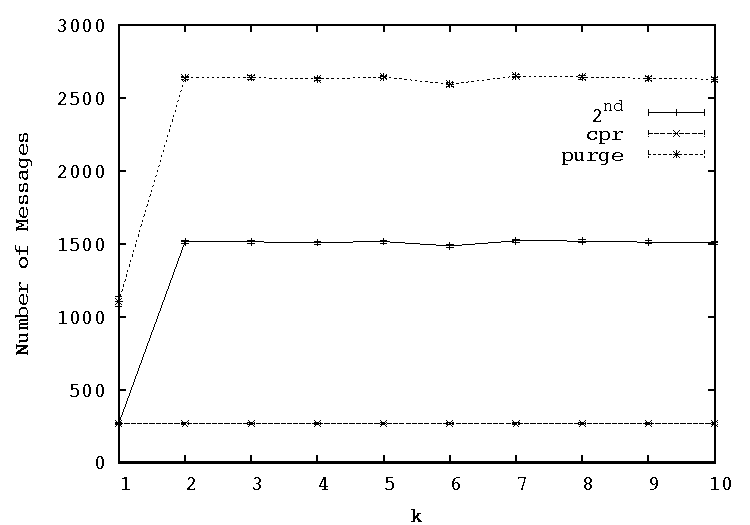
\includegraphics[width=0.32\textwidth]{figs/synch/msg15.pdf}}
\subfigure[{$p=0.25$, diameter=$2.99$}]{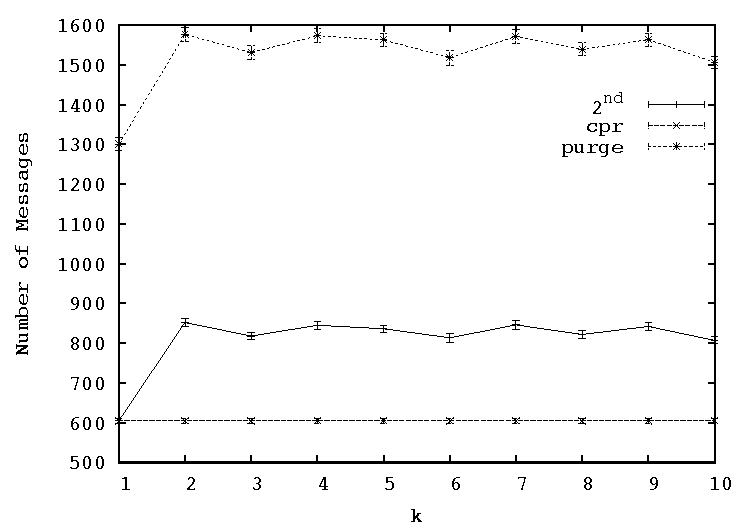
\includegraphics[width=0.32\textwidth]{figs/synch/msg25.pdf}}
\subfigure[{$p=0.50$, diameter=$2$}]{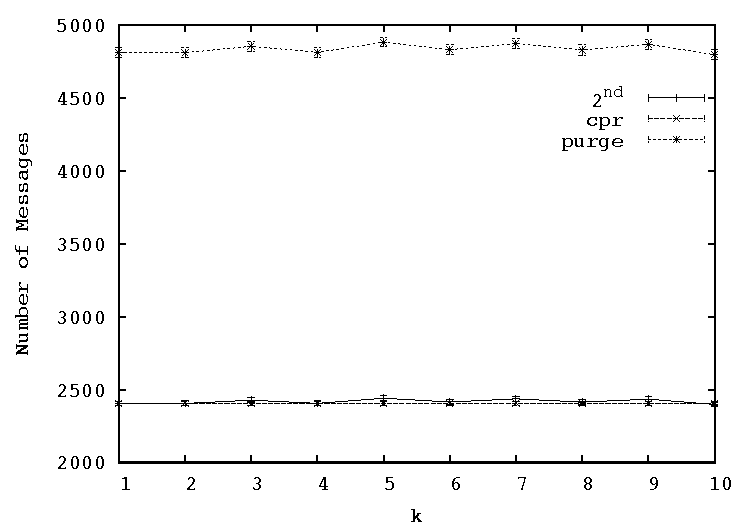
\includegraphics[width=0.32\textwidth]{figs/synch/msg50.pdf}}
%\subfigure[{Cumulative path cost decreases during the simulation}]{\includegraphics[width=0.49\textwidth]{figs/tsdecrease6.pdf}}
\caption{Message overhead for \er Graphs with Fixed Unit Link Weights generated over different $p$ values.}
\label{fig:msg}
\end{figure*}

\begin{figure*}[t]
\centering
\subfigure[{$p=0.05$, diameter=$6.14$}]{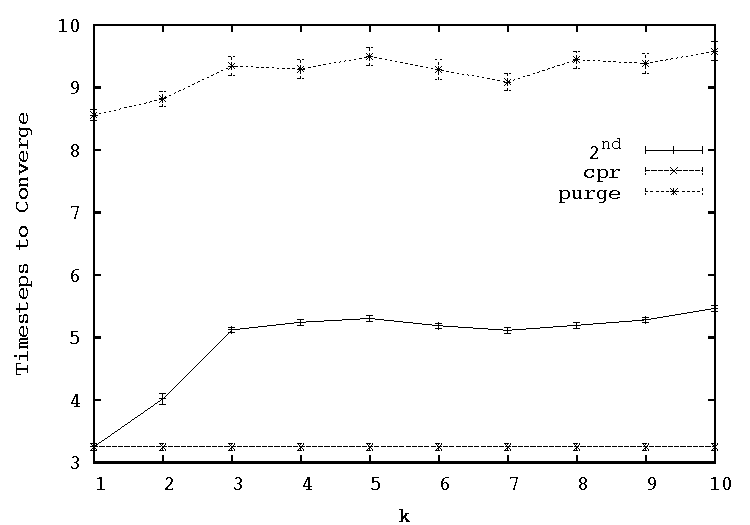
\includegraphics[width=0.32\textwidth]{figs/synch/epoch5.pdf}}
\subfigure[{$p=0.15$}, diamter=$3.01$]{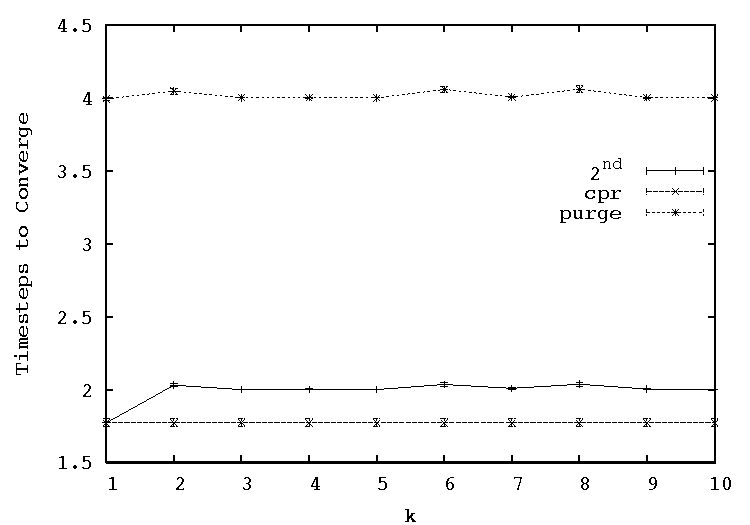
\includegraphics[width=0.32\textwidth]{figs/synch/epoch15.pdf}}
\subfigure[{$p=0.25$}, diameter=$2.99$]{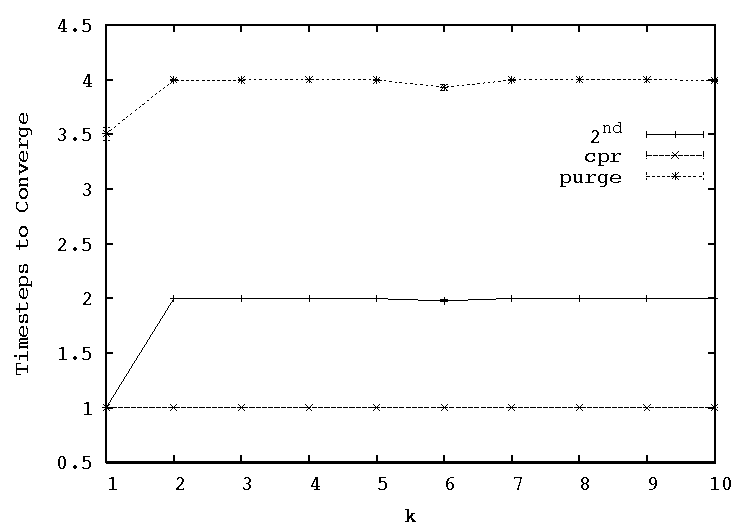
\includegraphics[width=0.32\textwidth]{figs/synch/epoch25.pdf}}
\subfigure[{$p=0.50$}, diameter=$2$]{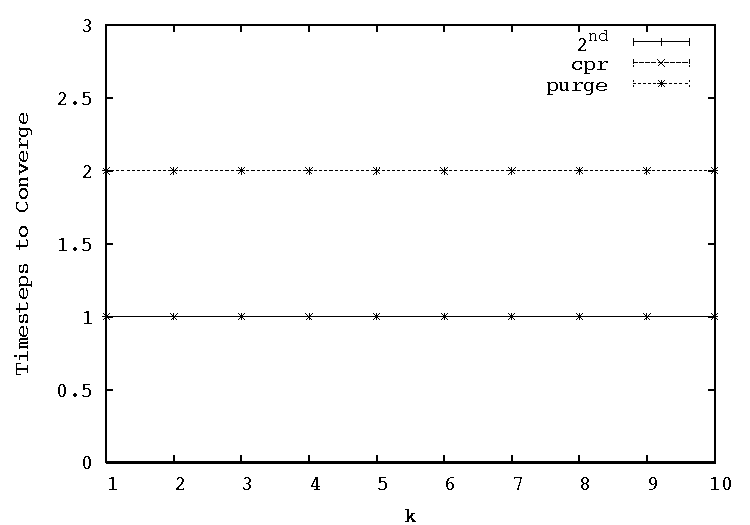
\includegraphics[width=0.32\textwidth]{figs/synch/epoch50.pdf}}
%\subfigure[{Cumulative path cost decreases during the simulation}]{\includegraphics[width=0.49\textwidth]{figs/tsdecrease6.pdf}}
\caption{Time overhead for \er Graphs with Fixed Unit Link Weights generated over different $p$ values.}
\label{fig:epoch}
\end{figure*} 




From Figure \ref{fig:msg}, we conclude that \cpr outperforms \purge and \second across all topologies. \cpr performs well because \badvector is removed using a single diffusing computation,  
while the other algorithms remove \badvector state through an iterative process.  \cprs's global state after rolling back is almost the same as the final recovered state.
%In other words, \cpr performs well because its global state  (recall we define the global state of the routers as the union of their local states) is almost the same as the final recovered state.
%Specifically, if we let $S'$ represent the global state after rolling back and let $S$ be the final recovered state, the only difference between $S$ and $S'$, is that $S'$ 
%contains state that depends directly or transitively on \oldvector while $S$ does not. 
%\cpr performs exactly the same as \second at $k=1$ because \second at $k=1$ also must only remove \oldvector state and uses the same iterative process as \cprs. 
%For this reason, across all $k$ values, \cpr performs exactly the same as \second at $k=1$.  {\bf note:} {\it may need to elaborate more here.}

\second recovery can be characterized as follows.  By Corollary 4 and 5 in Section \ref{subsec:trends}, distance values increase from their initial value until they 
reach their final (correct) value. Any intermediate, non-final, distance value uses \badvector or \oldvectors. Because \badvector and \oldvector no longer exist during recovery,
these intermediate values must correspond to routing loops.
%In this experiment, with \second distance estimates quickly count up to their final value.
Table \ref{tab:loop1} shows that there are few pairwise routing loops during \second recovery, indicating that \second distance values quickly count up to their final value.
{\footnote {\small We compute this metric as follows. After each simulation timestep, we count all pairwise routings loops over all source-destination pairs and then sum all of these values.}}
Although no pairwise routing loops exist during \purge recovery, \purge incurs overhead in its purge phase.  Roughly, $50\%$ of \purges's messages come from the \purge phase.
For these reasons, \purge has higher message overhead than \seconds.

Due to space limitations, we only show the time overhead for $p=.05$ (Figure \ref{fig:epoch}). The trends for time overhead match the trends we observed for message overhead. 
{\footnote {\small For the remaining experiments, we omit time overhead plots because time overhead follows the same trends as message overhead.}}

\begin{table}
\begin{center}
\begin{tabular}{l|l|l|l|l}
 & $k=1$&  $k=2$ & $k=3$ & $k=4-10$ \\
\hline
 Experiment 1, $p=0.05$  & $0$ & $14$ & $87$ &  $92$ \\
 Experiment 1, $p=0.15$  & $0$ & $7$&  $8$ & $9$ \\
 Experiment 2, $p=0.05$  & $554$ & $1303$ & $9239$ &  $12641$ \\
 %$p=\{0.15,0.25,0.50\}$  & $0$ & $0$&  $0$ & $0$ \\
\end{tabular}
\end{center}
\caption{Average number pairwise routing loops for \second in Experiment 1 and 2.}
%$p=.50$ for Experiment 1 is omitted because no pairwise routing loops are found across all $k$ values.} 
\label{tab:loop1}
\end{table}


\purge and \second message overhead increases with larger $k$. Larger $k$ implies more paths to repair, and therefore increased messaging.
For values of $k$ greater than a graph's diameter, the message overhead remains constant, as expected. 

%However, once $k$ is equal the graph diameter, $d$, the message overhead and number of epochs do not change for larger values of $k$ for a given topology. By definition, the graph diameter is
%the longest shortest path and so it follows that when $k > d$, each $v \in V'$ has a path less than $k$ hops to all destinations.  Therefore each $v$, does not use the $k$ hop path to \bads.
%For this reason, the message overhead (and number of epochs) do not change for $k>d$. {\bf todo verify if this is correct}

%Figure \ref{fig:compare} shows that for most values of $k$, if we do not count the epochs that occurred during \purges's purge phase 
%(e.g., only count \purges's discovery phase epochs), the resulting epoch omplexity is lower than \seconds's epoch complexity. When $k>2$, \second has higher epoch complexity 
%because the \infinity problem occurs with \second and not with \purges.  Table \ref{tab:loop1} shows that when $k>2$ there are pairwise routing loops during \second recovery, while

%The exception to this trend is when $k=1$ for all topologies and $k=2$ for $p=.05$: \purges's discovery phase epoch complexity is higher than \seconds's total epoch complexity. 
%In these cases, there are no or few pairwise routing loops for \seconds.  In this way, this is an ideal case for \second recovery. 
%Meanwhile, there are several cases in which distance values that previously used \oldvectors, which do not require messaging for \second but do for \purges.  
%Recall that \purge sets all distances that use \badvector or \oldvector to $\infty$ in its purge phase, so for \purge all distances using \oldvector must be recomputed. 
%With \seconds, many of these same distance values do not require re-computation: the actual path changes such as not to use \oldvector but the distance does not change because an 
%alternate path of the same distance is locally selected (since the distance does not change, no message is sent).




\subsubsection{Experiment 2 - \er Graphs with Fixed Link Costs and Random Link Weights}
\label{subsec:expt2}


The experimental setup is identical to Experiment 1 with one exception: link weights are selected uniformly at random between $[1,n]$ (rather than using 
fixed link weight of $50$).

Figure \ref{fig:msg-rand} show the message overhead across different $k$ for $p=.05$. We omit the figures for the other $p$ values because they follow the 
same trend as $p=.05$ \cite{Tech}.
In contrast to Experiment 1, \purge outperforms \second for most values of $k$. 
\second performs poorly because the \infinity problem: Table \ref{tab:loop1} shows the average number of pairwise routing loops, an indicator of the occurrence of \infinity problem.
No routing loops are found with \purges. \cpr performs well for the same reasons described in Section \ref{subsubsec:expt1}.  

\begin{figure*}[t]
\centering
\subfigure[{$p=0.05$, diameter=$6.14$}]{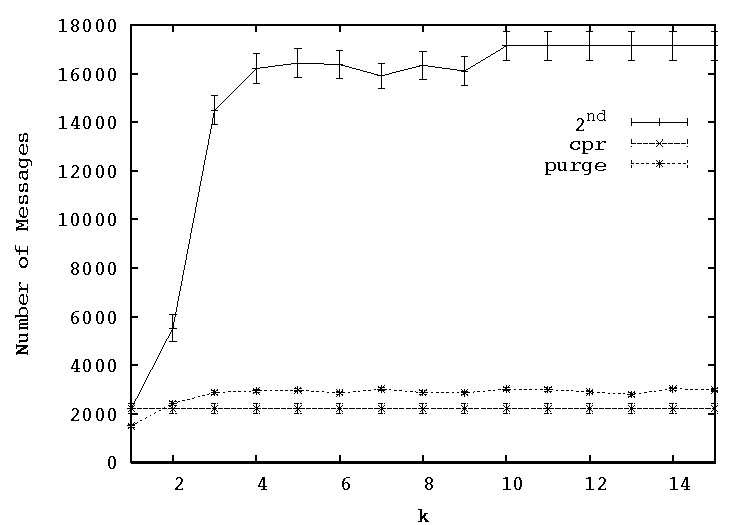
\includegraphics[width=0.32\textwidth]{figs/synch/msg-rand5.pdf}}
\subfigure[{$p=0.15$, diameter=$3.01$}]{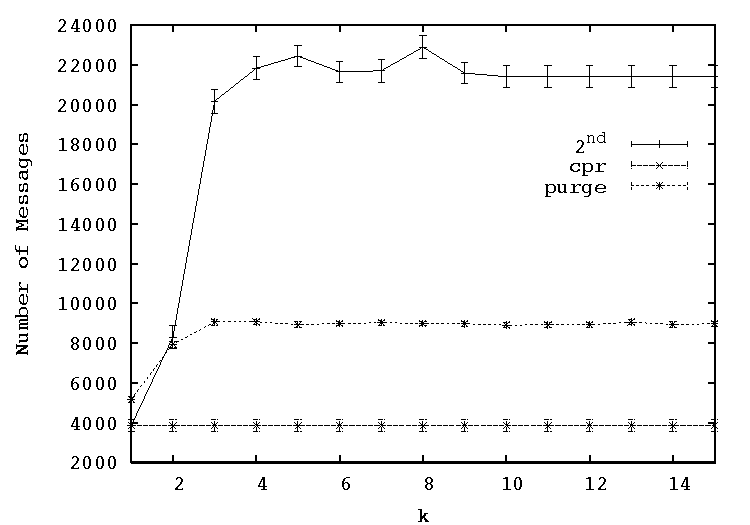
\includegraphics[width=0.32\textwidth]{figs/synch/msg-rand15.pdf}}
\subfigure[{$p=0.25$, diameter=$2.99$}]{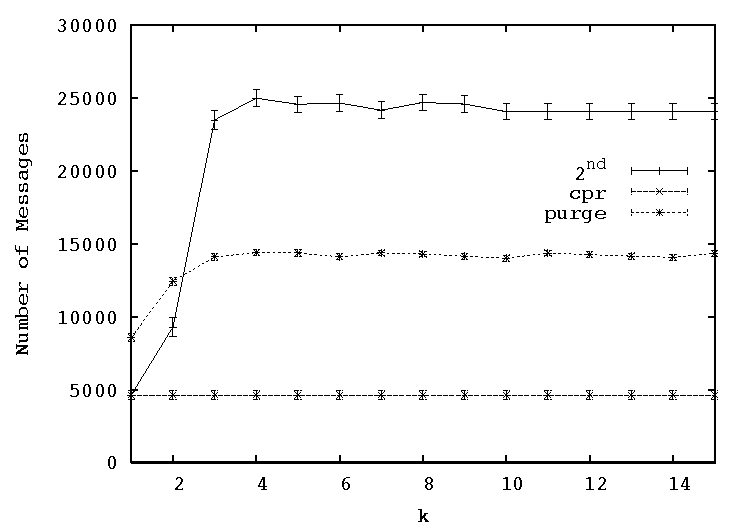
\includegraphics[width=0.32\textwidth]{figs/synch/msg-rand25.pdf}}
\subfigure[{$p=0.50$, diameter=$2$}]{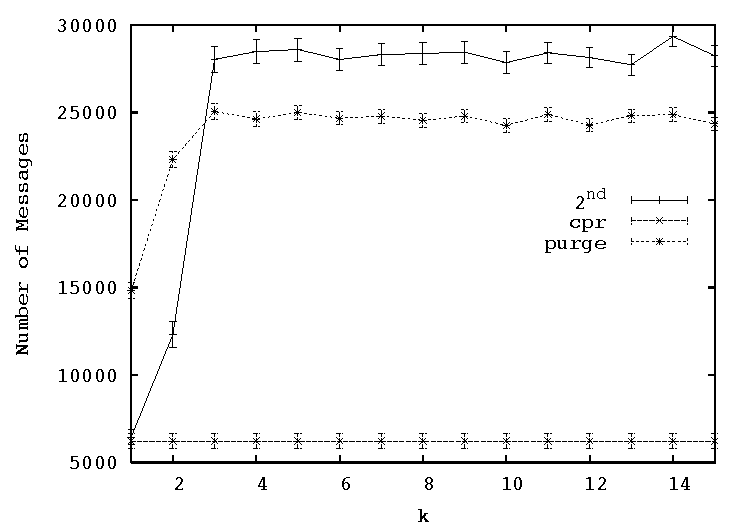
\includegraphics[width=0.32\textwidth]{figs/synch/msg-rand50.pdf}}
\caption{Message overhead for \er graph with link weights selected uniformly random from $[1,100]$}
\label{fig:msg-rand}
\end{figure*}

\begin{figure*}[t]
\centering
\subfigure[{$p=0.05$, diameter=$6.14$}]{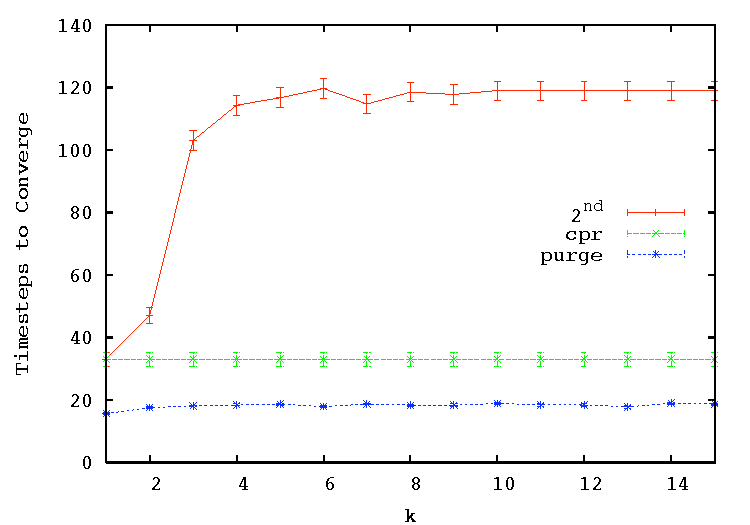
\includegraphics[width=0.32\textwidth]{figs/synch/epoch-rand5.pdf}}
\subfigure[{$p=0.15$, diameter=$3.01$}]{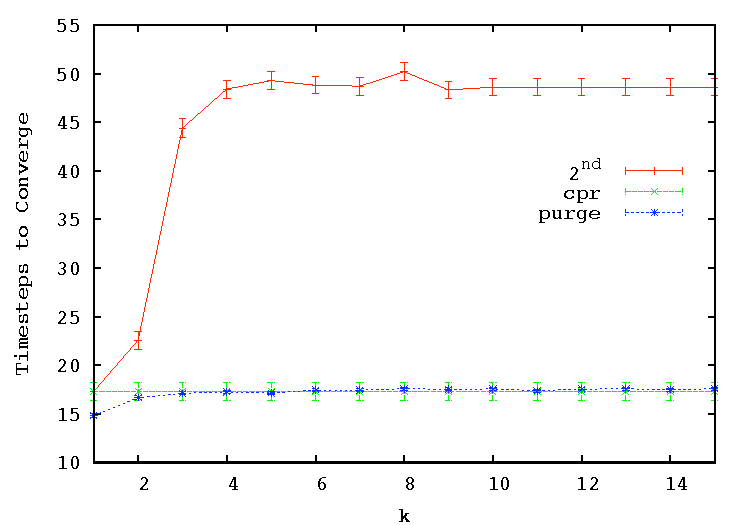
\includegraphics[width=0.32\textwidth]{figs/synch/epoch-rand15.pdf}}
\subfigure[{$p=0.25$, diameter=$2.99$}]{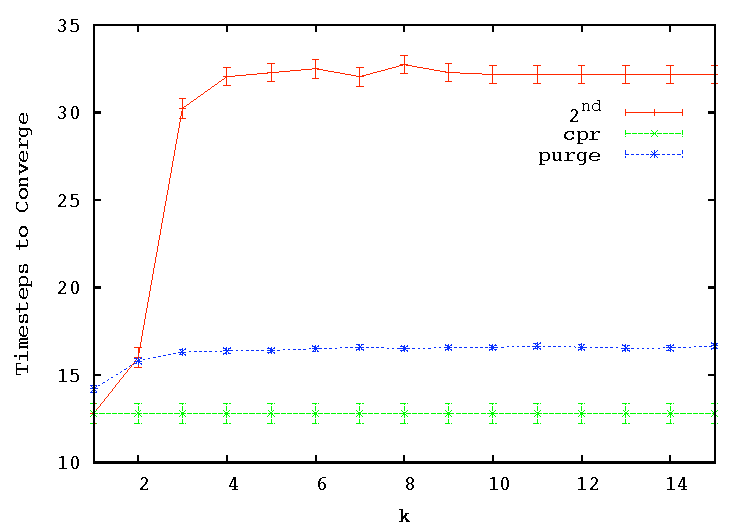
\includegraphics[width=0.32\textwidth]{figs/synch/epoch-rand25.pdf}}
\subfigure[{$p=0.50$, diameter=$2$}]{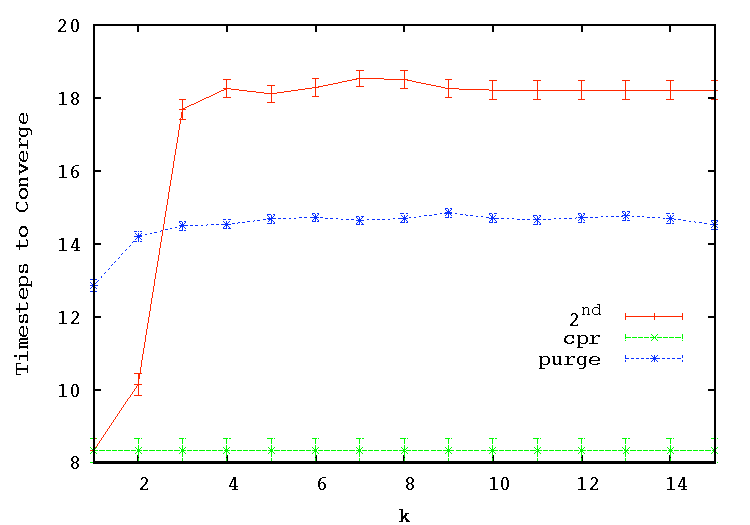
\includegraphics[width=0.32\textwidth]{figs/synch/epoch-rand50.pdf}}
%\subfigure[{Cumulative path cost decreases during the simulation}]{\includegraphics[width=0.49\textwidth]{figs/tsdecrease6.pdf}}
\caption{Time overhead for \er graph with link weights selected uniformly random from $[1,100]$}
\label{fig:epoch-rand}
\end{figure*} 




%Recall that in Experiment 1, no pairwise routing loops are found when $p=0.15,p=0.25,$ and $p=0.50$.  The only pairwise routing loops in Experiment 1 
%are found when $p=0.05$, where a maximum of only $100$ pairwise routing loops occur. For \purges, no pairwise routing loops were found. {\bf Self-note}: {\it verify}.

In addition, we counted the number of epochs in which at least one pairwise routing loop existed.  For \second (across all topologies), on average, all but the last three 
timesteps had at least one routing loop.  This suggests that the \infinity problem dominates the cost for \seconds. 
In some cases (e.g. $k=1$ for $p=.15$ and $p=.50$) \second performs better than \purges.  In these cases, \second has few routing loops.
%Table \ref{tab:loop} shows that there are fewer routing loops for small $k$. This is the case because with small $k$ there are fewer nodes using \badvectors. 

%The performance gap between \second and \purge shrinks with larger $p$ because with \second there are fewer routing loops with larger $p$.  
%This is consistent with our intuition:  larger $p$ values imply there are more alternate paths that do not use \badvectors.
%and thus routing loops are quickly exited because a low cost alternate path is used. 





\subsubsection{Experiment 3 - Internet-like Topologies}

\begin{figure*}[t]
\centering
\subfigure[{GT-ITM, diameter=$ $}]{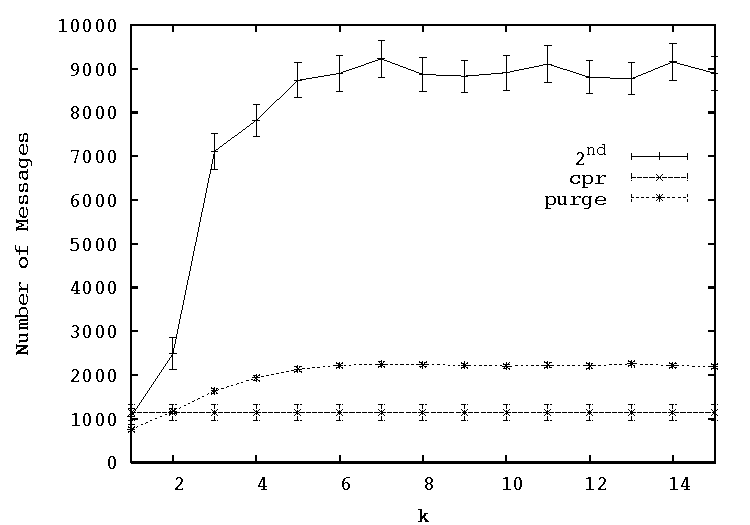
\includegraphics[width=0.32\textwidth]{figs/synch/msg-att.pdf}}
\subfigure[{Rocketfuel 6461, $n=141$, average node degree=$2.62$, diameter=$8$}]{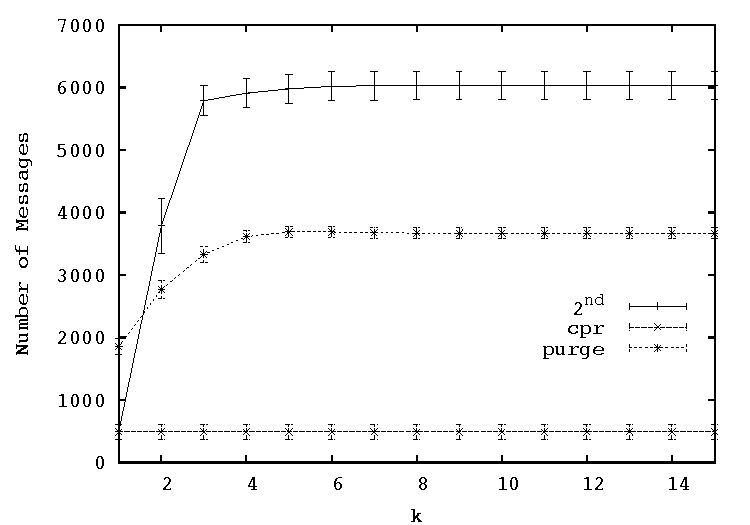
\includegraphics[width=0.32\textwidth]{figs/synch/msg6461.pdf}}
\subfigure[{Rocketfuel 3867, diameter=$ $}]{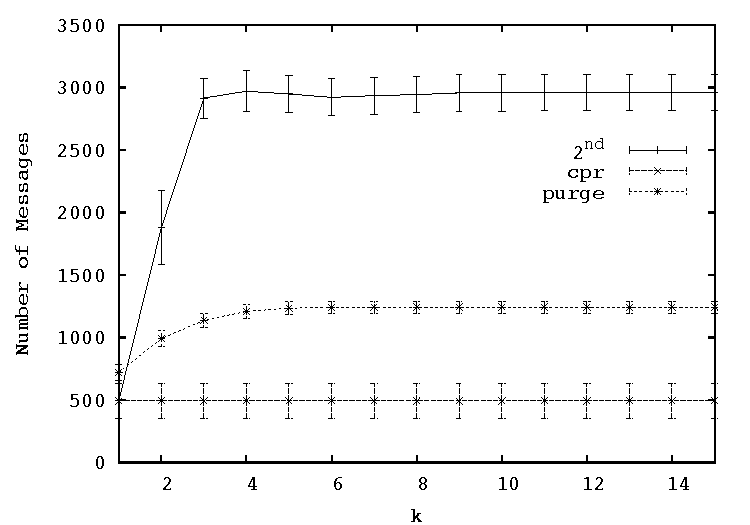
\includegraphics[width=0.32\textwidth]{figs/synch/msg3867.pdf}}
\caption{Internet-like graph message overhead}
\label{fig:msg-real}
\end{figure*}

\begin{figure*}[h]
\centering
\subfigure[{GT-ITM}]{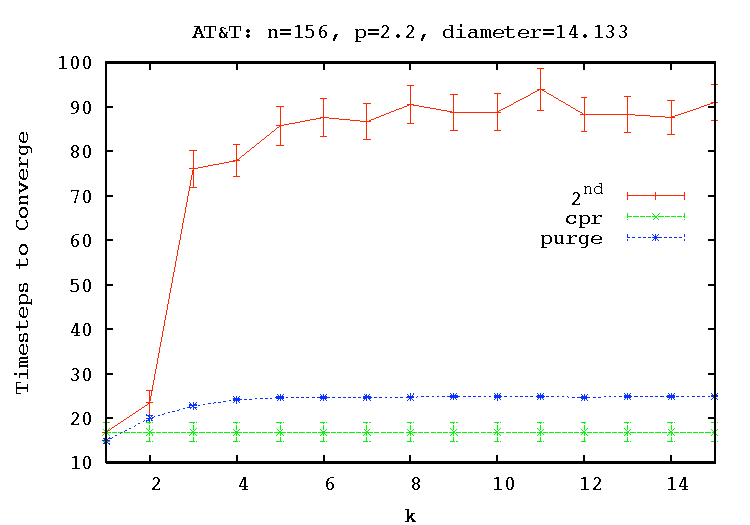
\includegraphics[width=0.32\textwidth]{figs/synch/att-epoch.pdf}}
\subfigure[{Rocketfuel 6461, $n=141$, average node degree=$2.62$, diameter=$12$}]{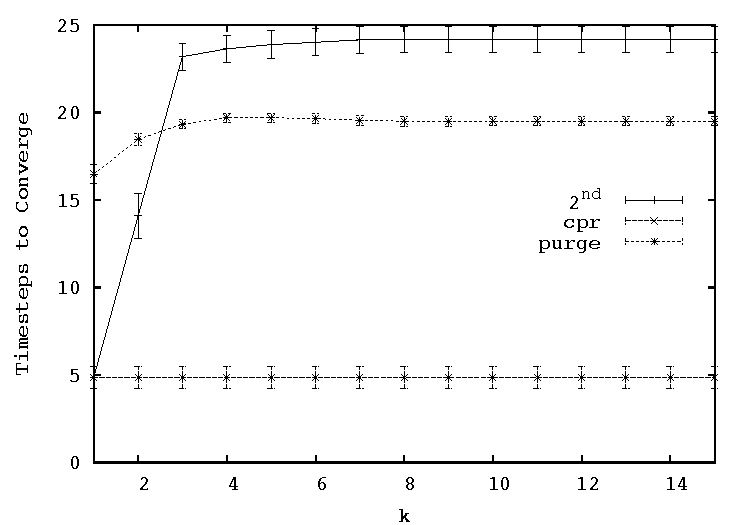
\includegraphics[width=0.32\textwidth]{figs/synch/rocket-epoch6461.pdf}}
\subfigure[{Rocketfuel 3867}]{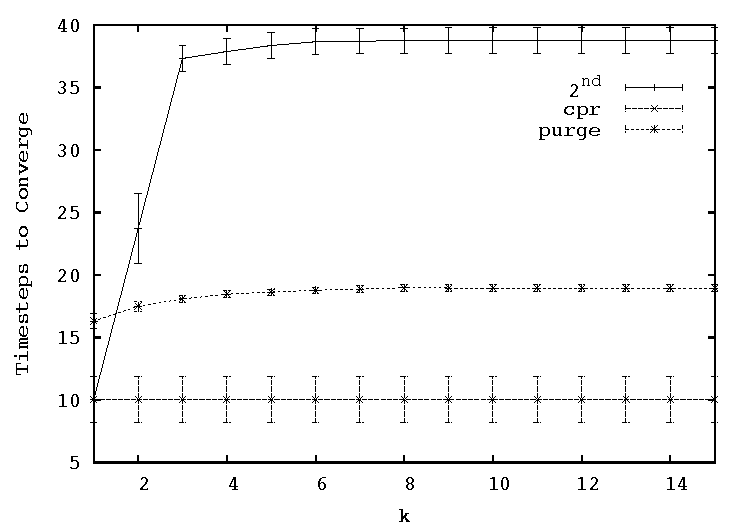
\includegraphics[width=0.32\textwidth]{figs/synch/rocket-epoch3867.pdf}}
%\subfigure[{Cumulative path cost decreases during the simulation}]{\includegraphics[width=0.49\textwidth]{figs/tsdecrease6.pdf}}
\caption{Number of epochs/timesteps for real graphs}
\label{fig:epoch-real}
\end{figure*} 





Thus far, we studied the performance of our recovery algorithms over \er graphs. Although unrealistic, these graphs provide us with useful intuition about the performance
of each algorithm. In this experiment, we simulate our algorithms over Internet-like topologies downloaded from the Rocketfuel website \cite{Rocketfuel} and generated using GT-ITM 
\cite{GT-ITM}.  The Rocketfuel topologies have inferred edge weights. For each Rocketfuel topology, we let each node be
the compromised node and average over all of these cases for each value of $k$.  For GT-ITM, we used the parameters specified in Heckmann et al \cite{Heckmann} to generate the $154$ node AT\&T topology
described in Section 4 of \cite{Heckmann}. For the GT-ITM topologies, we use the same criteria specified in Experiment 1 to generate each data point. 

The results, shown in Figure \ref{fig:msg-real}, follow the same pattern as in Experiment 2.  Due to space limitations, we only show the results for one 
representative topology.  The results for the other topologies follow the same pattern \cite{Tech}. In the cases where \second performs poorly,
the \infinity problem dominates the cost, as evidenced by the number of pairwise routing loops. In the few cases that \second performs better than \purges, there 
are few pairwise routing loops.



\subsection{Link Weight Change Experiments}
\label{subsec:change}

So far, we have evaluated our algorithms over different topologies with fixed link costs. We found that \cpr outperforms the other algorithms because \cpr removes false
routing state with a single diffusing computation, rather than using an iterative process like \second and \purges.  In the next 
two experiments we evaluate our algorithms over graphs with changing link costs. We introduce link cost changes between the time \bad is compromised and when \bad is discovered 
(e.g. during $[t',t]$). 
In particular, there are $\lambda$ link cost changes per timestep, where $\lambda$ is deterministic. 
To create a link cost change event, we modify links uniformly at random (except for all $(v,\bar{v})$ links). % where $v \in V'$ and $v \in adj(\bar{v})$.
The new link cost is selected uniformly at random from $[1,n]$. 

\subsubsection{Experiment 4}

Except for $\lambda$, our experimental setup is identical to the one in Experiment 2. We let $\lambda = \{1,4,8\}$. In order to isolate the effects of link costs changes,
we assume that \cpr checkpoints at each timestep.

Due to space constraints, we only show results for $p=.05$ in Figure \ref{fig:lc-p05}.  
{\footnote {\small Our experiments for different $p$ values, yield the same trends.  Refer to our technical report for more details \cite{Tech}.}}
\purge yields the lowest message overhead, but only slightly lower than \cprs. 
\cprs's message overhead increases with larger $k$ because there are more link cost change events to process. After \cpr rolls back, it must process all \lcd events. 
In contrast, \second and \purge process some of the \lcd events during the interval $[t',t]$.  In our experimental setup, these messages are not counted because 
they do not occur in Step 4 of our simulation scenario described in Section \ref{sec:eval}.

Our analysis further indicates that \second performance suffers because of the \infinity problem. %\purge and \second must 
The gap between \second and the other algorithms shrinks as $\lambda$ increases because as $\lambda$ increases, link cost changes have a larger effect on message overhead.



\begin{figure*}[t]
\centering
\subfigure[{$p=0.05$, diameter=$6.14, \lambda=1$}]{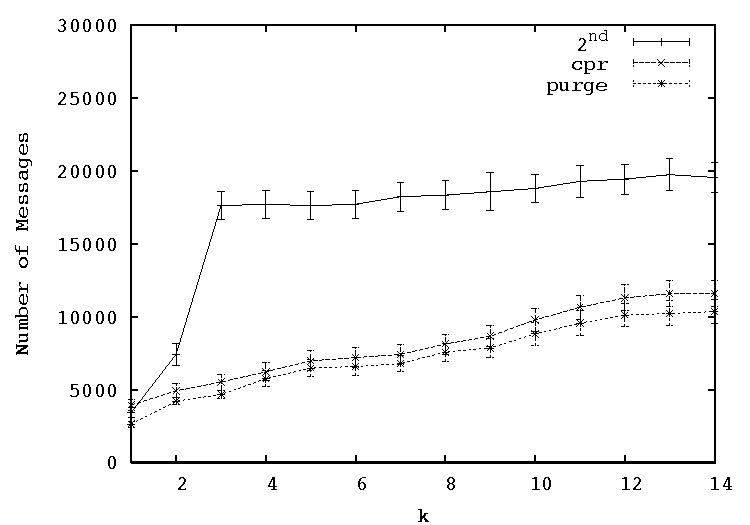
\includegraphics[width=0.32\textwidth]{figs/synch/p05-lc1.pdf}}
\subfigure[{$p=0.05$, diameter=$6.14, \lambda=2$}]{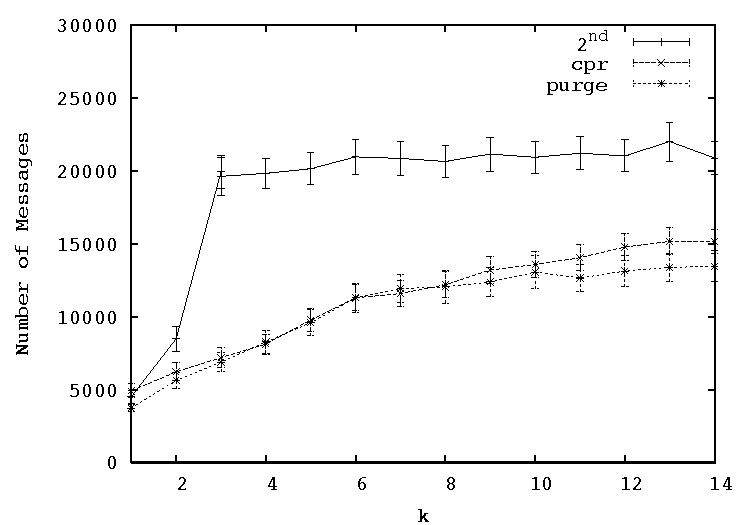
\includegraphics[width=0.32\textwidth]{figs/synch/p05-lc2.pdf}}
\subfigure[{$p=0.05$, diameter=$6.14,\lambda=4$}]{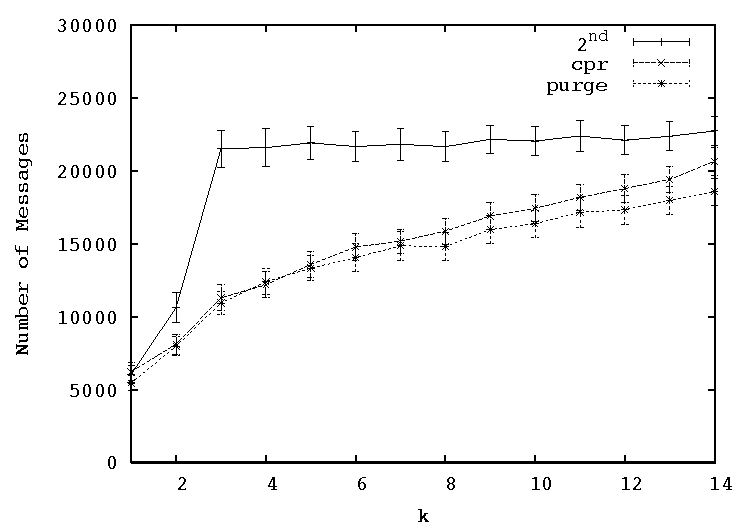
\includegraphics[width=0.32\textwidth]{figs/synch/p05-lc4.pdf}}
\subfigure[{$p=0.05$, diameter=$6.14, \lambda=8$}]{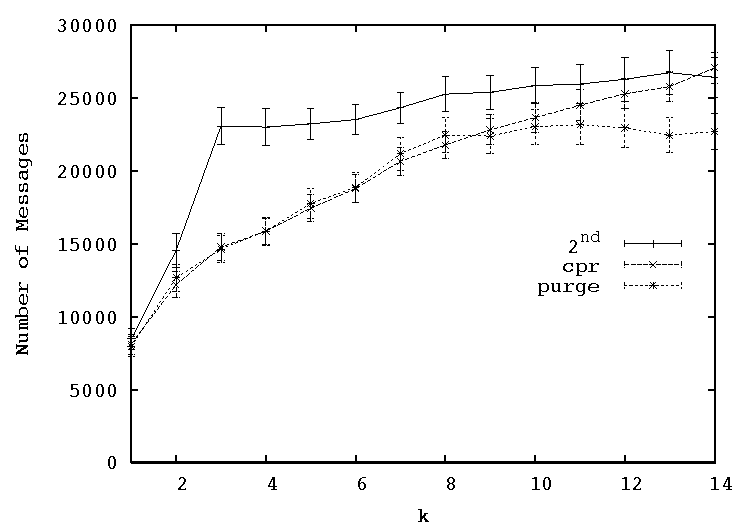
\includegraphics[width=0.32\textwidth]{figs/synch/p05-lc8.pdf}}
%\subfigure[{Cumulative path cost decreases during the simulation}]{\includegraphics[width=0.49\textwidth]{figs/tsdecrease6.pdf}}
\caption{Message overhead for $p=0.05$ \er with link weights selected uniformly random with different $\lambda$ values.}
\label{fig:lc-p05}
\end{figure*} 


\subsubsection{Experiment 5}

In this experiment we study the trade-off between message overhead and storage overhead for \cprs. To this end, we vary the frequency at which \cpr checkpoints and fix 
the interval $[t'-t]$. We assume at each timestep before $t$, \lcd events occur at rate $\lambda$. Otherwise, our experimental setup is the same as Experiment 4.

Due to space constraints, we only display a single plot. Figure \ref{fig:lc-fixk} shows the results for an \er graph with link weights selected uniformly at random between $[1,n]$,
$n=100$, $p=.05$, $\lambda=4$ and $k=2$. We plot message overhead against the number of timesteps \cpr must rollback, $z$. \cprs's message overhead increases with larger $z$ 
because as $z$ increases there are more \lcd events to process. \second and \purge have constant message overhead because they operate independent of $z$.

We conclude that as the frequency of \cpr snapshots decreases, \cpr incurs higher message overhead.  Therefore, when choosing the frequency of checkpoints,
the trade-off between storage and message overhead must be carefully considered. 


\begin{figure}[t]
\centering
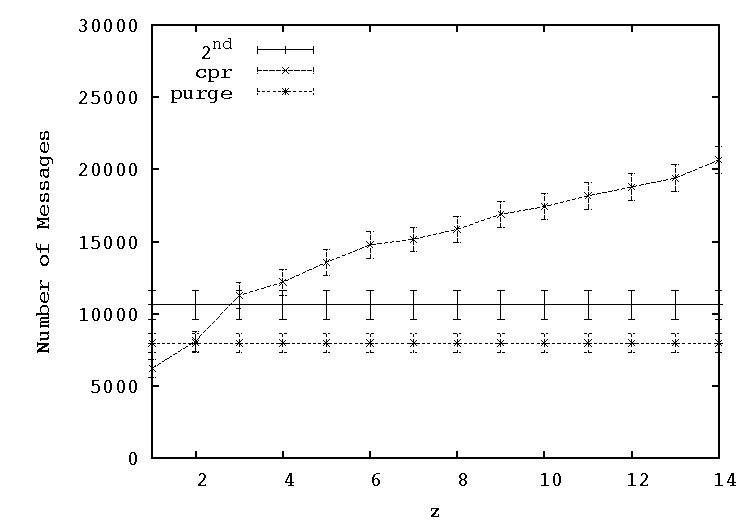
\includegraphics[scale=.35]{figs/synch/p05-k4.pdf}
%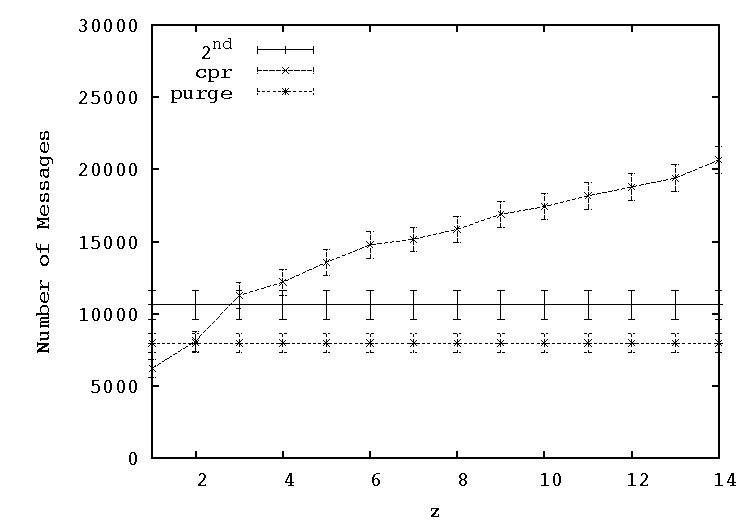
\includegraphics[width=.30\textwidth]{figs/synch/p05-k4.pdf}
\caption{Message overhead for $p=0.05$ \er with link weights selected uniformly random with different $\lambda$ values. $z$ refers to the number of timesteps \cpr must 
rollback.}
\label{fig:lc-fixk}
\end{figure} 


\subsection{Summary}
\label{subsec:discuss}

Our results show that for graphs with fixed link costs, \cpr yields the lowest message and time overhead. \cpr benefits from removing false state with a single
diffusing computation. However, \cpr has storage overhead, requires loosely synchronized clocks, and requires the time \bad was compromised be identified.

\seconds's performance is determined by the \infinity problem. In this case of \er graphs with fixed unit link weights, the \infinity problem was minimal, 
helping \second perform better than \purges. \purge avoids the \infinity problem by globally invalidating false state.  Therefore in cases where the \infinity problem is 
significant, \purge outperforms \seconds.

When considering graphs with changing link costs, \cprs's performance suffers because it must process all valid link cost changes that occurred since \bad was compromised.
Meanwhile, \second and \purge make use of computations that preceded the injection of false state, that do not depend on false routing state. However, \seconds's performance degrades 
because of the \infinity problem.  \purge eliminated the \infinity problem and therefore yields the best performance over topologies with changing link costs.

Finally, we found that an additional challenge with \cpr is setting the parameter which determines the rate of checkpointing. 
More frequent checkpointing yields lower message and time overhead at the cost of more storage overhead. Ultimately, application specific factors must be considered
when setting this parameter. 

\begin{comment}

\begin{enumerate}

	\item Our results show that for graphs with fixed link costs, \cpr yields the lowest message and time overhead. \cpr benefits from removing false state with a single
diffusing computation. However, \cpr has storage overhead, requires loosely synchronized clocks, and requires the time \bad was compromised be identified.

	\item \seconds's performance is determined by the \infinity problem. In this case of \er graphs with fixed unit link weights, the \infinity problem was minimal, 
helping \second perform better than \purges. \purge avoids the \infinity problem by globally invalidating false state.  Therefore in cases where the \infinity problem is 
significant, \purge outperforms \seconds.

	\item When considering graphs with changing link costs, \cprs's performance suffers because it must process all valid link cost changes that occurred since \bad was compromised.
Meanwhile, \second and \purge make use of computations that preceded the injection of false state, that do not depend on false routing state. However, \seconds's performance degrades 
because of the \infinity problem.  \purge eliminated the \infinity problem and therefore yields the best performance over topologies with changing link costs.

	\item Finally, we found that an additional challenge with \cpr is setting the parameter which determines the rate of checkpointing. 
More frequent checkpointing yields lower message and time overhead at the cost of more storage overhead. Ultimately, application specific factors must be considered
when setting this parameter. 

\end{enumerate}

\end{comment}
